%%
%% kit-prog-tutorial
%%
%% Slides for my Java programming tutorial at KIT using LaTeX beamer.
%%
%% Copyright (c) 2015-2016 YouniS Bensalah <younis.bensalah@gmail.com>
%%
%% This work is released to the public domain.
%% For the full copyright and license information, please view the LICENSE file.
%%

\documentclass[18pt]{beamer}

\usepackage{templates/beamerthemekit}

\usepackage[utf8]{inputenc}
\usepackage{hyperref}
\usepackage{listings}

%\titleimage{bauplan}
%\titleimage{greendrop}
%\titleimage{bluedrop}
%\titleimage{pinkdrop}
%\titleimage{fall}
%\titleimage{forestleaves}
%\titleimage{coloredtrees}
\titleimage{road}
%\titleimage{sortedleaves}
%\titleimage{topviewtrees}

\newcommand{\tagline}{Hello World}

\title[Programmieren\hspace{2.5pt}--\hspace{2.5pt}\tagline]{\tagline}
\subtitle{Programmieren~\textbar~Tutorium 32}

\author{YouniS Bensalah}
\date{31. Oktober 2016}

\institute{Chair for Software Design and Quality}

\usepackage[citestyle=authoryear,bibstyle=numeric,hyperref,backend=biber]{biblatex}
\addbibresource{templates/example.bib}
\bibhang1em

\begin{document}

% remove annoying figure prefix in caption
\setbeamertemplate{caption}{\raggedright\insertcaption\par}

\selectlanguage{english}

\begin{frame}
    \titlepage
\end{frame}

% \begin{frame}{Heute}
%     \tableofcontents
% \end{frame}

\section{Organisatorisches}

\subsection{Hi}

\begin{frame}{Hi}
    \begin{itemize}
        \item \textbf{Younis Bensalah}
        \item Bachelor Informatik
        \item 5. Semester
        \item \url{younis.bensalah@gmail.com}
    \end{itemize}
\end{frame}

\subsection{Übungsbetrieb}

\begin{frame}{Folien, Übungsblätter etc.}
    \begin{itemize}
        \item \textbf{Vorlesungsunterlagen und Übungsblätter}
        \begin{itemize}
            \item \url{https://sdqweb.ipd.kit.edu/wiki/Vorlesung_Programmieren_WS16/17}
        \end{itemize}

        \vspace{.1in}

        \item \textbf{Tutoriumsfolien}
        \begin{itemize}
            \item Im ILIAS unter \textit{Tutorien}
            \item \url{https://ilias.studium.kit.edu/ilias.php?ref_id=614188&cmd=view&cmdClass=ilrepositorygui&cmdNode=75&baseClass=ilrepositorygui}
        \end{itemize}
    \end{itemize}
\end{frame}

\begin{frame}{Modul Programmieren auf Twitter\ldots}
    \begin{figure}
        
\includegraphics[scale=.4]{img/modulprogtwitter.png}
    \end{figure}
\end{frame}

\begin{frame}{Disclaimer}
    \begin{itemize}
        \item \textbf{Frist: \alert{06.11.2016}}
        \item Unterschreiben und in den Programmieren-Briefkasten werfen
        \item Info-Bau (50.34) 1. UG
    \end{itemize}
\end{frame}

\begin{frame}{Übungsblätter und Präsenzübung}
    \begin{block}{Übungsblätter}
        \begin{itemize}
            \item \textbf{5} Übungsblätter
            \item \textbf{2} Wochen Bearbeitungszeit
            \item Abgabe (exklusiv) über Praktomat
            \item Ungefähr \textbf{100} Punkte insgesamt (20 je Blatt)
            \item $>$\textbf{50}$\%$ hinreichend
        \end{itemize}
    \end{block}

    \pause

    \begin{block}{Präsenzübung}
        \begin{itemize}
            \item Schriftliche Prüfung ($\sim$20 Minuten)
            \item $>$\textbf{75}$\%$ hinreichend
            \item Findet am \textbf{25.01.2017} statt
        \end{itemize}
    \end{block}


\end{frame}

\begin{frame}{Übungsschein}
    \begin{itemize}
        \item \textbf{Übungsschein = \alert{5}} Übungsblätter + \textbf{\alert{1}} Präsenzübung
        \pause
        \item \alert{Vorraussetzung für Abschlussaufgaben}
        \pause
        \item Übungsblätter oder Präsenzübung \textit{nicht} bestanden
        \begin{itemize}
            \item kein Schein, beides wiederholen
        \end{itemize}
        \pause
        \item Ausnahme: Rücktritt von Präsenzübung aus triftigem Grund
        \begin{itemize}
            \item kein Schein, nur Präsenzübung wiederholen
        \end{itemize}
    \end{itemize}

\end{frame}

\begin{frame}{Orientierungsprüfung}
    \begin{itemize}
        \item \textbf{Modul Programmieren} ist \textbf{Orientierungsprüfung}!
        \begin{itemize}
            \item Bis zum 2. Semester antreten
            \item Bis zum 3. Semester bestehen
        \end{itemize}

    \end{itemize}
\end{frame}


\subsection{Praktomat}

\begin{frame}{Praktomat}
    \begin{block}{Praktomat}
        \begin{itemize}
            \item Hier gebt ihr die Übungsaufgaben ab
            \item Zugang mit KIT-Account (uxxxx)
            \item \alert{Umgehend anmelden!}
            \item \url{https://praktomat.cs.kit.edu/2016_WS}
        \end{itemize}
    \end{block}

\end{frame}


\subsection{VPN}

\begin{frame}{VPN}
    \begin{itemize}
        \item \textbf{\alert{Praktomat nur aus dem KIT-Netz erreichbar!}}
        \item Möglichkeit, von außerhalb (z.B. von zu Hause) eine Verbindung mit dem KIT-Netz herzustellen
        \item Zugang mit KIT-Account (uxxxx)
        \item Anleitung hier: \url{https://www.scc.kit.edu/dienste/vpn.php}
    \end{itemize}
\end{frame}


\subsection{ILIAS}

\begin{frame}{ILIAS}
    \begin{block}{ILIAS}
        \begin{itemize}
            \item \textbf{Forum zu Vorlesung und Übungsaufgaben}
            \item Login via KIT-Account (uxxxx)
            \item Kurs \textit{Programmieren} beitreten
            \item \url{https://ilias.studium.kit.edu}
        \end{itemize}
    \end{block}
\end{frame}


\section{Java}

\subsection{Java Development Kit}

\subsection{Vom Quelltext zum laufenden Programm}

\subsection{Code-Editor}

\appendix

\beginbackup

\begin{frame}{Fragen?}
    \begin{figure}
        
\includegraphics[scale=.3]{img/fragen.jpg}
    \end{figure}
\end{frame}

\begin{frame}{Bis nächste Woche!}
    \begin{figure}
        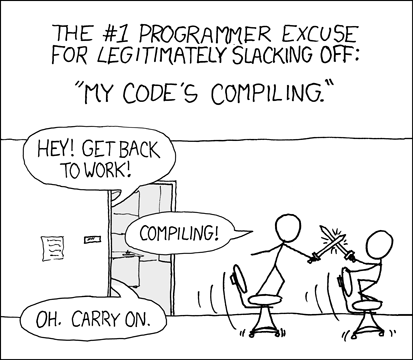
\includegraphics[scale=.4]{img/compiling.png}
        \caption{\footnotesize{xkcd.com}}
    \end{figure}
\end{frame}

\backupend

\end{document}
